\section{September 16, 2026}
% Based on pages 1--4 of 551-0916&0918.pdf.

We study the stability domains of explicit Runge--Kutta methods and
use them to choose time steps. The examples show two different
obstructions: rapidly decaying modes can force very small steps, and
an undamped oscillator can become unstable under discretization.
Throughout, \(A\) denotes the matrix in the differential equation;
\(\mathsf{A}=(a_{ij})\) denotes the Runge--Kutta coefficient matrix.

\subsection{Continuous stability and discrete stability}

For a constant matrix \(A\), the solution of \(x'=Ax\) is
\(x(t)=e^{tA}x(0)\). Recall the two spectral criteria:
\[
\begin{array}{c|c|c}
 &\text{asymptotic stability}&\text{stability (boundedness)}\\ \hline
 x'=Ax&\operatorname{Re}\lambda<0&\operatorname{Re}\lambda\leq0\\
 x_{n+1}=Gx_n&|\mu|<1&|\mu|\leq1
\end{array}
\]
Here the conditions apply to every \(\lambda\in\sigma(A)\) and
\(\mu\in\sigma(G)\), respectively. In the boundedness column,
eigenvalues on the boundary must also be \emph{semisimple}: every
associated Jordan block must have size one. Algebraic multiplicity
one is sufficient, but is not necessary.

\begin{figure}[htbp]
\centering
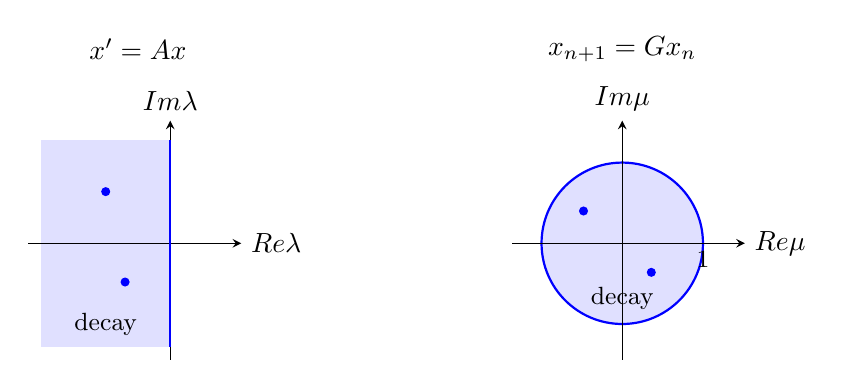
\begin{tikzpicture}[scale=.82,>=stealth]
 \begin{scope}
  \fill[blue!12] (-2,-1.6) rectangle (0,1.6);
  \draw[->] (-2.2,0)--(1.1,0) node[right] {\(\operatorname{Re}\lambda\)};
  \draw[->] (0,-1.8)--(0,1.9) node[above] {\(\operatorname{Im}\lambda\)};
  \draw[blue,thick] (0,-1.6)--(0,1.6);
  \fill[blue] (-1,.8) circle (2pt); \fill[blue] (-.7,-.6) circle (2pt);
  \node at (-1,-1.25) {\small decay};
  \node at (-.5,3.0) {\(x'=Ax\)};
 \end{scope}
 \begin{scope}[xshift=7cm]
  \filldraw[fill=blue!12,draw=blue,thick] (0,0) circle (1.25);
  \draw[->] (-1.7,0)--(1.9,0) node[right] {\(\operatorname{Re}\mu\)};
  \draw[->] (0,-1.8)--(0,1.9) node[above] {\(\operatorname{Im}\mu\)};
  \fill[blue] (-.6,.5) circle (2pt); \fill[blue] (.45,-.45) circle (2pt);
  \node at (1.25,-.25) {\small 1};
  \node at (0,-.85) {\small decay};
  \node at (0,3.0) {\(x_{n+1}=Gx_n\)};
 \end{scope}
\end{tikzpicture}
\caption{The open left half-plane governs continuous decay; the open
unit disk governs discrete decay. Boundary eigenvalues require the
additional Jordan-block condition for boundedness.}
\label{fig:continuous-discrete-sep-16}
\end{figure}

For an explicit RK method applied with a fixed step \(\tau>0\),
\[
 x_{n+1}=R(\tau A)x_n,
 \qquad
 \sigma(R(\tau A))=\{R(\tau\lambda):\lambda\in\sigma(A)\}.
\]
For example, the eigenvector identity
\(R(\tau A)v=R(\tau\lambda)v\) follows from \(Av=\lambda v\).
Triangularizing \(A\) proves the full spectral mapping identity even
when \(A\) is not diagonalizable. Consequently,
\[
 \rho(R(\tau A))=\max_{\lambda\in\sigma(A)}|R(\tau\lambda)|,
\]
and strict inequality \(\rho(R(\tau A))<1\) characterizes asymptotic
stability of the numerical evolution.

\subsection{The stability domain in the complex plane}

\begin{definition}[Stability domain]
 For the scalar test equation \(y'=\lambda y\), put \(z=\tau\lambda\)
 and write \(y_{n+1}=R(z)y_n\). We use the notation
 \begin{equation}\label{eq:closed-stability-domain-sep-16}
  \mathcal D=\{z\in\bb{C}:|R(z)|\leq1\},
  \qquad
  \mathcal S=\{z\in\bb{C}:|R(z)|<1\}.
 \end{equation}
 Thus \(\mathcal D\) describes bounded scalar iterates, and
 \(\mathcal S\) describes decay. For a rational stability function,
 these sets contain only points where the function is defined.
\end{definition}

The handwritten notes use the non-strict convention \(\mathcal D\);
\(\mathcal S\) agrees with the strict convention used in the previous
lecture. In particular, \(R(0)=1\), so \(0\in\mathcal D\) but
\(0\notin\mathcal S\). To reproduce decay of a linear system, every
scaled eigenvalue \(\tau\lambda\) must belong to \(\mathcal S\).
Membership in \(\mathcal D\) alone does not settle a matrix problem
with defective boundary eigenvalues.

\subsubsection{Forward Euler}

Here \(R_1(z)=1+z\). Writing \(z=x+iy\),
\[
 |R_1(z)|\leq1
 \quad\Longleftrightarrow\quad
 (x+1)^2+y^2\leq1.
\]
The domain is the closed disk of radius one centered at \(-1\).
For a negative real eigenvalue,
\begin{equation}\label{eq:euler-real-bound-sep-16}
 |1+\tau\lambda|<1
 \quad\Longleftrightarrow\quad
 0<\tau<\frac{2}{|\lambda|}.
\end{equation}
At the upper endpoint the amplification factor is \(-1\): the scalar
solution alternates without decaying.

\subsubsection{Two, three, and four stages}

An explicit two-stage method of order two has
\[
 R_2(z)=1+z+\frac{z^2}{2}.
\]
Its boundary can be plotted using
\[
 \left(1+x+\frac{x^2-y^2}{2}\right)^2+y^2(1+x)^2=1.
\]
On the negative real axis, \(R_2(-r)=1-r+r^2/2\) is positive and is
less than one exactly when \(0<r<2\). Thus its real stability interval
is the same as forward Euler's, despite its higher order.

The standard three-stage, third-order method and classical RK4 have
\[
 R_3(z)=1+z+\frac{z^2}{2}+\frac{z^3}{6},
 \qquad
 R_4(z)=1+z+\frac{z^2}{2}+\frac{z^3}{6}+\frac{z^4}{24}.
\]
Their strict negative-real stability intervals are approximately
\[
 (-2.512745,0)\quad\text{and}\quad(-2.785294,0),
\]
respectively. The following
plots are computed from \(|R_j(z)|=1\), rather than schematic ovals.

\begin{figure}[htbp]
\centering
% Boundaries track the roots of R(z)=exp(i theta), theta in [0,2 pi].
% The root branches are joined into closed curves.
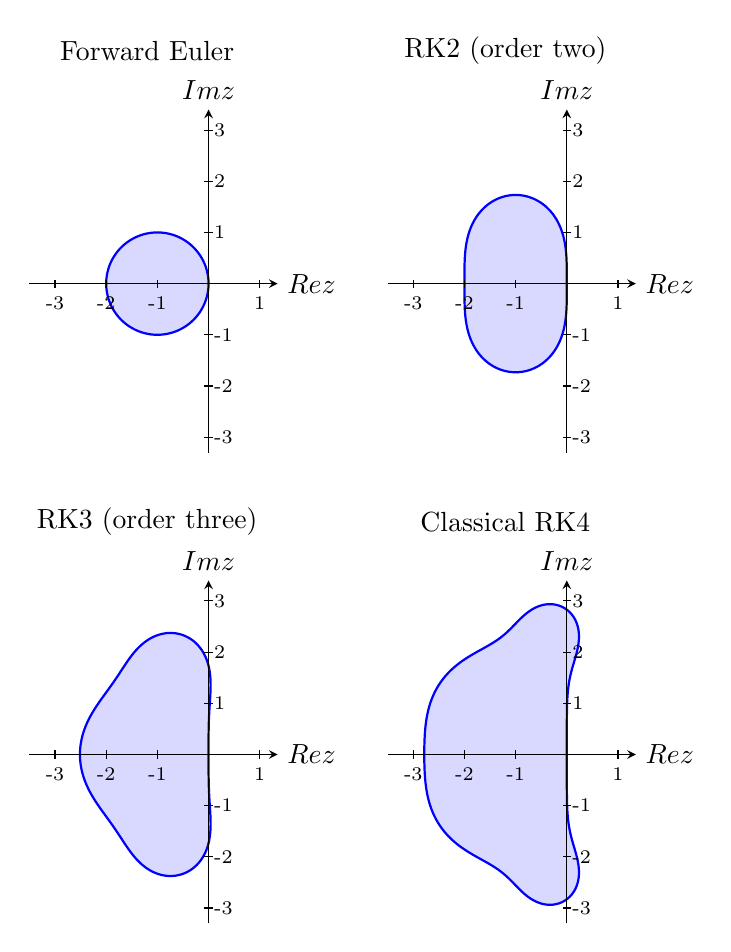
\begin{tikzpicture}[scale=.65,>=stealth]
\begin{scope}[shift={(0,0)}]
\node at (-1.2,4.55) {Forward Euler};
\filldraw[fill=blue!15,draw=blue,thick] plot coordinates {
(0.00000,0.00000) (-0.00077,0.03926) (-0.00308,0.07846) (-0.00693,0.11754) (-0.01231,0.15643) (-0.01921,0.19509)
(-0.02763,0.23345) (-0.03754,0.27144) (-0.04894,0.30902) (-0.06181,0.34612) (-0.07612,0.38268) (-0.09186,0.41866)
(-0.10899,0.45399) (-0.12750,0.48862) (-0.14736,0.52250) (-0.16853,0.55557) (-0.19098,0.58779) (-0.21468,0.61909)
(-0.23959,0.64945) (-0.26568,0.67880) (-0.29289,0.70711) (-0.32120,0.73432) (-0.35055,0.76041) (-0.38091,0.78532)
(-0.41221,0.80902) (-0.44443,0.83147) (-0.47750,0.85264) (-0.51138,0.87250) (-0.54601,0.89101) (-0.58134,0.90814)
(-0.61732,0.92388) (-0.65388,0.93819) (-0.69098,0.95106) (-0.72856,0.96246) (-0.76655,0.97237) (-0.80491,0.98079)
(-0.84357,0.98769) (-0.88246,0.99307) (-0.92154,0.99692) (-0.96074,0.99923) (-1.00000,1.00000) (-1.03926,0.99923)
(-1.07846,0.99692) (-1.11754,0.99307) (-1.15643,0.98769) (-1.19509,0.98079) (-1.23345,0.97237) (-1.27144,0.96246)
(-1.30902,0.95106) (-1.34612,0.93819) (-1.38268,0.92388) (-1.41866,0.90814) (-1.45399,0.89101) (-1.48862,0.87250)
(-1.52250,0.85264) (-1.55557,0.83147) (-1.58779,0.80902) (-1.61909,0.78532) (-1.64945,0.76041) (-1.67880,0.73432)
(-1.70711,0.70711) (-1.73432,0.67880) (-1.76041,0.64945) (-1.78532,0.61909) (-1.80902,0.58779) (-1.83147,0.55557)
(-1.85264,0.52250) (-1.87250,0.48862) (-1.89101,0.45399) (-1.90814,0.41866) (-1.92388,0.38268) (-1.93819,0.34612)
(-1.95106,0.30902) (-1.96246,0.27144) (-1.97237,0.23345) (-1.98079,0.19509) (-1.98769,0.15643) (-1.99307,0.11754)
(-1.99692,0.07846) (-1.99923,0.03926) (-2.00000,0.00000) (-1.99923,-0.03926) (-1.99692,-0.07846) (-1.99307,-0.11754)
(-1.98769,-0.15643) (-1.98079,-0.19509) (-1.97237,-0.23345) (-1.96246,-0.27144) (-1.95106,-0.30902) (-1.93819,-0.34612)
(-1.92388,-0.38268) (-1.90814,-0.41866) (-1.89101,-0.45399) (-1.87250,-0.48862) (-1.85264,-0.52250) (-1.83147,-0.55557)
(-1.80902,-0.58779) (-1.78532,-0.61909) (-1.76041,-0.64945) (-1.73432,-0.67880) (-1.70711,-0.70711) (-1.67880,-0.73432)
(-1.64945,-0.76041) (-1.61909,-0.78532) (-1.58779,-0.80902) (-1.55557,-0.83147) (-1.52250,-0.85264) (-1.48862,-0.87250)
(-1.45399,-0.89101) (-1.41866,-0.90814) (-1.38268,-0.92388) (-1.34612,-0.93819) (-1.30902,-0.95106) (-1.27144,-0.96246)
(-1.23345,-0.97237) (-1.19509,-0.98079) (-1.15643,-0.98769) (-1.11754,-0.99307) (-1.07846,-0.99692) (-1.03926,-0.99923)
(-1.00000,-1.00000) (-0.96074,-0.99923) (-0.92154,-0.99692) (-0.88246,-0.99307) (-0.84357,-0.98769) (-0.80491,-0.98079)
(-0.76655,-0.97237) (-0.72856,-0.96246) (-0.69098,-0.95106) (-0.65388,-0.93819) (-0.61732,-0.92388) (-0.58134,-0.90814)
(-0.54601,-0.89101) (-0.51138,-0.87250) (-0.47750,-0.85264) (-0.44443,-0.83147) (-0.41221,-0.80902) (-0.38091,-0.78532)
(-0.35055,-0.76041) (-0.32120,-0.73432) (-0.29289,-0.70711) (-0.26568,-0.67880) (-0.23959,-0.64945) (-0.21468,-0.61909)
(-0.19098,-0.58779) (-0.16853,-0.55557) (-0.14736,-0.52250) (-0.12750,-0.48862) (-0.10899,-0.45399) (-0.09186,-0.41866)
(-0.07612,-0.38268) (-0.06181,-0.34612) (-0.04894,-0.30902) (-0.03754,-0.27144) (-0.02763,-0.23345) (-0.01921,-0.19509)
(-0.01231,-0.15643) (-0.00693,-0.11754) (-0.00308,-0.07846) (-0.00077,-0.03926) (0.00000,0.00000)
} -- cycle;
\draw[->] (-3.5,0)--(1.35,0) node[right] {\(\operatorname{Re}z\)};
\draw[->] (0,-3.3)--(0,3.4) node[above] {\(\operatorname{Im}z\)};
\foreach \x in {-3,-2,-1,1} \draw (\x,.08)--(\x,-.08) node[below] {\scriptsize \x};
\foreach \y in {-3,-2,-1,1,2,3} \draw (.08,\y)--(-.08,\y) node[right] {\scriptsize \y};
\end{scope}
\begin{scope}[shift={(7,0)}]
\node at (-1.2,4.55) {RK2 (order two)};
\filldraw[fill=blue!15,draw=blue,thick] plot coordinates {
(-2.00000,0.00000) (-2.00000,-0.03926) (-2.00000,-0.07846) (-1.99998,-0.11754) (-1.99993,-0.15645) (-1.99982,-0.19513)
(-1.99964,-0.23353) (-1.99934,-0.27162) (-1.99891,-0.30936) (-1.99829,-0.34671) (-1.99747,-0.38365) (-1.99641,-0.42017)
(-1.99507,-0.45624) (-1.99343,-0.49185) (-1.99147,-0.52700) (-1.98915,-0.56167) (-1.98645,-0.59586) (-1.98336,-0.62957)
(-1.97986,-0.66280) (-1.97592,-0.69555) (-1.97156,-0.72781) (-1.96674,-0.75959) (-1.96146,-0.79089) (-1.95571,-0.82171)
(-1.94950,-0.85204) (-1.94281,-0.88190) (-1.93565,-0.91128) (-1.92800,-0.94019) (-1.91988,-0.96861) (-1.91128,-0.99655)
(-1.90221,-1.02402) (-1.89266,-1.05100) (-1.88264,-1.07751) (-1.87216,-1.10353) (-1.86121,-1.12907) (-1.84981,-1.15412)
(-1.83796,-1.17869) (-1.82566,-1.20276) (-1.81292,-1.22634) (-1.79975,-1.24943) (-1.78615,-1.27202) (-1.77214,-1.29411)
(-1.75771,-1.31569) (-1.74289,-1.33677) (-1.72767,-1.35734) (-1.71206,-1.37739) (-1.69608,-1.39693) (-1.67973,-1.41595)
(-1.66302,-1.43444) (-1.64596,-1.45241) (-1.62856,-1.46985) (-1.61082,-1.48675) (-1.59277,-1.50312) (-1.57441,-1.51894)
(-1.55575,-1.53423) (-1.53679,-1.54896) (-1.51756,-1.56315) (-1.49805,-1.57678) (-1.47829,-1.58986) (-1.45827,-1.60238)
(-1.43802,-1.61433) (-1.41754,-1.62573) (-1.39684,-1.63655) (-1.37594,-1.64680) (-1.35484,-1.65649) (-1.33356,-1.66559)
(-1.31210,-1.67412) (-1.29049,-1.68207) (-1.26872,-1.68944) (-1.24682,-1.69623) (-1.22479,-1.70244) (-1.20264,-1.70805)
(-1.18039,-1.71308) (-1.15804,-1.71752) (-1.13562,-1.72137) (-1.11312,-1.72464) (-1.09057,-1.72730) (-1.06797,-1.72938)
(-1.04533,-1.73086) (-1.02267,-1.73175) (-1.00000,-1.73205) (-0.97733,-1.73175) (-0.95467,-1.73086) (-0.93203,-1.72938)
(-0.90943,-1.72730) (-0.88688,-1.72464) (-0.86438,-1.72137) (-0.84196,-1.71752) (-0.81961,-1.71308) (-0.79736,-1.70805)
(-0.77521,-1.70244) (-0.75318,-1.69623) (-0.73128,-1.68944) (-0.70951,-1.68207) (-0.68790,-1.67412) (-0.66644,-1.66559)
(-0.64516,-1.65649) (-0.62406,-1.64680) (-0.60316,-1.63655) (-0.58246,-1.62573) (-0.56198,-1.61433) (-0.54173,-1.60238)
(-0.52171,-1.58986) (-0.50195,-1.57678) (-0.48244,-1.56315) (-0.46321,-1.54896) (-0.44425,-1.53423) (-0.42559,-1.51894)
(-0.40723,-1.50312) (-0.38918,-1.48675) (-0.37144,-1.46985) (-0.35404,-1.45241) (-0.33698,-1.43444) (-0.32027,-1.41595)
(-0.30392,-1.39693) (-0.28794,-1.37739) (-0.27233,-1.35734) (-0.25711,-1.33677) (-0.24229,-1.31569) (-0.22786,-1.29411)
(-0.21385,-1.27202) (-0.20025,-1.24943) (-0.18708,-1.22634) (-0.17434,-1.20276) (-0.16204,-1.17869) (-0.15019,-1.15412)
(-0.13879,-1.12907) (-0.12784,-1.10353) (-0.11736,-1.07751) (-0.10734,-1.05100) (-0.09779,-1.02402) (-0.08872,-0.99655)
(-0.08012,-0.96861) (-0.07200,-0.94019) (-0.06435,-0.91128) (-0.05719,-0.88190) (-0.05050,-0.85204) (-0.04429,-0.82171)
(-0.03854,-0.79089) (-0.03326,-0.75959) (-0.02844,-0.72781) (-0.02408,-0.69555) (-0.02014,-0.66280) (-0.01664,-0.62957)
(-0.01355,-0.59586) (-0.01085,-0.56167) (-0.00853,-0.52700) (-0.00657,-0.49185) (-0.00493,-0.45624) (-0.00359,-0.42017)
(-0.00253,-0.38365) (-0.00171,-0.34671) (-0.00109,-0.30936) (-0.00066,-0.27162) (-0.00036,-0.23353) (-0.00018,-0.19513)
(-0.00007,-0.15645) (-0.00002,-0.11754) (-0.00000,-0.07846) (-0.00000,-0.03926) (0.00000,0.00000) (-0.00000,0.03926)
(-0.00000,0.07846) (-0.00002,0.11754) (-0.00007,0.15645) (-0.00018,0.19513) (-0.00036,0.23353) (-0.00066,0.27162)
(-0.00109,0.30936) (-0.00171,0.34671) (-0.00253,0.38365) (-0.00359,0.42017) (-0.00493,0.45624) (-0.00657,0.49185)
(-0.00853,0.52700) (-0.01085,0.56167) (-0.01355,0.59586) (-0.01664,0.62957) (-0.02014,0.66280) (-0.02408,0.69555)
(-0.02844,0.72781) (-0.03326,0.75959) (-0.03854,0.79089) (-0.04429,0.82171) (-0.05050,0.85204) (-0.05719,0.88190)
(-0.06435,0.91128) (-0.07200,0.94019) (-0.08012,0.96861) (-0.08872,0.99655) (-0.09779,1.02402) (-0.10734,1.05100)
(-0.11736,1.07751) (-0.12784,1.10353) (-0.13879,1.12907) (-0.15019,1.15412) (-0.16204,1.17869) (-0.17434,1.20276)
(-0.18708,1.22634) (-0.20025,1.24943) (-0.21385,1.27202) (-0.22786,1.29411) (-0.24229,1.31569) (-0.25711,1.33677)
(-0.27233,1.35734) (-0.28794,1.37739) (-0.30392,1.39693) (-0.32027,1.41595) (-0.33698,1.43444) (-0.35404,1.45241)
(-0.37144,1.46985) (-0.38918,1.48675) (-0.40723,1.50312) (-0.42559,1.51894) (-0.44425,1.53423) (-0.46321,1.54896)
(-0.48244,1.56315) (-0.50195,1.57678) (-0.52171,1.58986) (-0.54173,1.60238) (-0.56198,1.61433) (-0.58246,1.62573)
(-0.60316,1.63655) (-0.62406,1.64680) (-0.64516,1.65649) (-0.66644,1.66559) (-0.68790,1.67412) (-0.70951,1.68207)
(-0.73128,1.68944) (-0.75318,1.69623) (-0.77521,1.70244) (-0.79736,1.70805) (-0.81961,1.71308) (-0.84196,1.71752)
(-0.86438,1.72137) (-0.88688,1.72464) (-0.90943,1.72730) (-0.93203,1.72938) (-0.95467,1.73086) (-0.97733,1.73175)
(-1.00000,1.73205) (-1.02267,1.73175) (-1.04533,1.73086) (-1.06797,1.72938) (-1.09057,1.72730) (-1.11312,1.72464)
(-1.13562,1.72137) (-1.15804,1.71752) (-1.18039,1.71308) (-1.20264,1.70805) (-1.22479,1.70244) (-1.24682,1.69623)
(-1.26872,1.68944) (-1.29049,1.68207) (-1.31210,1.67412) (-1.33356,1.66559) (-1.35484,1.65649) (-1.37594,1.64680)
(-1.39684,1.63655) (-1.41754,1.62573) (-1.43802,1.61433) (-1.45827,1.60238) (-1.47829,1.58986) (-1.49805,1.57678)
(-1.51756,1.56315) (-1.53679,1.54896) (-1.55575,1.53423) (-1.57441,1.51894) (-1.59277,1.50312) (-1.61082,1.48675)
(-1.62856,1.46985) (-1.64596,1.45241) (-1.66302,1.43444) (-1.67973,1.41595) (-1.69608,1.39693) (-1.71206,1.37739)
(-1.72767,1.35734) (-1.74289,1.33677) (-1.75771,1.31569) (-1.77214,1.29411) (-1.78615,1.27202) (-1.79975,1.24943)
(-1.81292,1.22634) (-1.82566,1.20276) (-1.83796,1.17869) (-1.84981,1.15412) (-1.86121,1.12907) (-1.87216,1.10353)
(-1.88264,1.07751) (-1.89266,1.05100) (-1.90221,1.02402) (-1.91128,0.99655) (-1.91988,0.96861) (-1.92800,0.94019)
(-1.93565,0.91128) (-1.94281,0.88190) (-1.94950,0.85204) (-1.95571,0.82171) (-1.96146,0.79089) (-1.96674,0.75959)
(-1.97156,0.72781) (-1.97592,0.69555) (-1.97986,0.66280) (-1.98336,0.62957) (-1.98645,0.59586) (-1.98915,0.56167)
(-1.99147,0.52700) (-1.99343,0.49185) (-1.99507,0.45624) (-1.99641,0.42017) (-1.99747,0.38365) (-1.99829,0.34671)
(-1.99891,0.30936) (-1.99934,0.27162) (-1.99964,0.23353) (-1.99982,0.19513) (-1.99993,0.15645) (-1.99998,0.11754)
(-2.00000,0.07846) (-2.00000,0.03926) (-2.00000,0.00000)
} -- cycle;
\draw[->] (-3.5,0)--(1.35,0) node[right] {\(\operatorname{Re}z\)};
\draw[->] (0,-3.3)--(0,3.4) node[above] {\(\operatorname{Im}z\)};
\foreach \x in {-3,-2,-1,1} \draw (\x,.08)--(\x,-.08) node[below] {\scriptsize \x};
\foreach \y in {-3,-2,-1,1,2,3} \draw (.08,\y)--(-.08,\y) node[right] {\scriptsize \y};
\end{scope}
\begin{scope}[shift={(0,-9.2)}]
\node at (-1.2,4.55) {RK3 (order three)};
\filldraw[fill=blue!15,draw=blue,thick] plot coordinates {
(-1.50000,1.93649) (-1.51521,1.91662) (-1.53043,1.89627) (-1.54568,1.87544) (-1.56097,1.85414) (-1.57631,1.83237)
(-1.59172,1.81014) (-1.60723,1.78746) (-1.62283,1.76434) (-1.63857,1.74079) (-1.65445,1.71682) (-1.67049,1.69247)
(-1.68671,1.66775) (-1.70312,1.64269) (-1.71975,1.61731) (-1.73659,1.59167) (-1.75366,1.56578) (-1.77097,1.53969)
(-1.78850,1.51344) (-1.80626,1.48707) (-1.82424,1.46062) (-1.84240,1.43413) (-1.86075,1.40765) (-1.87924,1.38120)
(-1.89784,1.35481) (-1.91654,1.32852) (-1.93529,1.30234) (-1.95405,1.27630) (-1.97279,1.25040) (-1.99148,1.22466)
(-2.01007,1.19908) (-2.02854,1.17367) (-2.04686,1.14841) (-2.06499,1.12332) (-2.08292,1.09837) (-2.10060,1.07357)
(-2.11803,1.04891) (-2.13519,1.02438) (-2.15205,0.99997) (-2.16860,0.97566) (-2.18482,0.95145) (-2.20071,0.92733)
(-2.21625,0.90329) (-2.23144,0.87933) (-2.24626,0.85542) (-2.26071,0.83157) (-2.27478,0.80776) (-2.28847,0.78399)
(-2.30177,0.76025) (-2.31468,0.73654) (-2.32720,0.71285) (-2.33931,0.68918) (-2.35103,0.66552) (-2.36234,0.64186)
(-2.37325,0.61821) (-2.38376,0.59455) (-2.39385,0.57090) (-2.40354,0.54724) (-2.41282,0.52357) (-2.42169,0.49989)
(-2.43015,0.47621) (-2.43820,0.45251) (-2.44584,0.42880) (-2.45306,0.40507) (-2.45988,0.38134) (-2.46628,0.35758)
(-2.47227,0.33382) (-2.47784,0.31004) (-2.48300,0.28625) (-2.48775,0.26245) (-2.49209,0.23863) (-2.49602,0.21480)
(-2.49953,0.19096) (-2.50262,0.16711) (-2.50531,0.14326) (-2.50758,0.11939) (-2.50944,0.09552) (-2.51089,0.07165)
(-2.51192,0.04777) (-2.51254,0.02388) (-2.51275,-0.00000) (-2.51254,-0.02388) (-2.51192,-0.04777) (-2.51089,-0.07165)
(-2.50944,-0.09552) (-2.50758,-0.11939) (-2.50531,-0.14326) (-2.50262,-0.16711) (-2.49953,-0.19096) (-2.49602,-0.21480)
(-2.49209,-0.23863) (-2.48775,-0.26245) (-2.48300,-0.28625) (-2.47784,-0.31004) (-2.47227,-0.33382) (-2.46628,-0.35758)
(-2.45988,-0.38134) (-2.45306,-0.40507) (-2.44584,-0.42880) (-2.43820,-0.45251) (-2.43015,-0.47621) (-2.42169,-0.49989)
(-2.41282,-0.52357) (-2.40354,-0.54724) (-2.39385,-0.57090) (-2.38376,-0.59455) (-2.37325,-0.61821) (-2.36234,-0.64186)
(-2.35103,-0.66552) (-2.33931,-0.68918) (-2.32720,-0.71285) (-2.31468,-0.73654) (-2.30177,-0.76025) (-2.28847,-0.78399)
(-2.27478,-0.80776) (-2.26071,-0.83157) (-2.24626,-0.85542) (-2.23144,-0.87933) (-2.21625,-0.90329) (-2.20071,-0.92733)
(-2.18482,-0.95145) (-2.16860,-0.97566) (-2.15205,-0.99997) (-2.13519,-1.02438) (-2.11803,-1.04891) (-2.10060,-1.07357)
(-2.08292,-1.09837) (-2.06499,-1.12332) (-2.04686,-1.14841) (-2.02854,-1.17367) (-2.01007,-1.19908) (-1.99148,-1.22466)
(-1.97279,-1.25040) (-1.95405,-1.27630) (-1.93529,-1.30234) (-1.91654,-1.32852) (-1.89784,-1.35481) (-1.87924,-1.38120)
(-1.86075,-1.40765) (-1.84240,-1.43413) (-1.82424,-1.46062) (-1.80626,-1.48707) (-1.78850,-1.51344) (-1.77097,-1.53969)
(-1.75366,-1.56578) (-1.73659,-1.59167) (-1.71975,-1.61731) (-1.70312,-1.64269) (-1.68671,-1.66775) (-1.67049,-1.69247)
(-1.65445,-1.71682) (-1.63857,-1.74079) (-1.62283,-1.76434) (-1.60723,-1.78746) (-1.59172,-1.81014) (-1.57631,-1.83237)
(-1.56097,-1.85414) (-1.54568,-1.87544) (-1.53043,-1.89627) (-1.51521,-1.91662) (-1.50000,-1.93649) (-1.48479,-1.95589)
(-1.46957,-1.97481) (-1.45433,-1.99325) (-1.43906,-2.01122) (-1.42375,-2.02871) (-1.40840,-2.04574) (-1.39301,-2.06230)
(-1.37756,-2.07840) (-1.36205,-2.09403) (-1.34649,-2.10921) (-1.33086,-2.12394) (-1.31517,-2.13821) (-1.29942,-2.15204)
(-1.28360,-2.16542) (-1.26772,-2.17836) (-1.25177,-2.19087) (-1.23575,-2.20294) (-1.21967,-2.21457) (-1.20353,-2.22578)
(-1.18733,-2.23657) (-1.17107,-2.24692) (-1.15475,-2.25686) (-1.13838,-2.26638) (-1.12196,-2.27549) (-1.10548,-2.28418)
(-1.08896,-2.29245) (-1.07240,-2.30032) (-1.05580,-2.30778) (-1.03916,-2.31484) (-1.02249,-2.32149) (-1.00579,-2.32774)
(-0.98906,-2.33359) (-0.97231,-2.33905) (-0.95555,-2.34410) (-0.93877,-2.34877) (-0.92198,-2.35303) (-0.90519,-2.35691)
(-0.88839,-2.36040) (-0.87160,-2.36350) (-0.85482,-2.36621) (-0.83805,-2.36853) (-0.82129,-2.37047) (-0.80456,-2.37203)
(-0.78785,-2.37321) (-0.77117,-2.37401) (-0.75452,-2.37442) (-0.73792,-2.37446) (-0.72136,-2.37413) (-0.70485,-2.37341)
(-0.68839,-2.37233) (-0.67199,-2.37087) (-0.65565,-2.36904) (-0.63938,-2.36684) (-0.62319,-2.36427) (-0.60707,-2.36134)
(-0.59103,-2.35803) (-0.57508,-2.35436) (-0.55922,-2.35033) (-0.54346,-2.34593) (-0.52780,-2.34118) (-0.51225,-2.33606)
(-0.49681,-2.33058) (-0.48148,-2.32474) (-0.46628,-2.31855) (-0.45120,-2.31200) (-0.43626,-2.30509) (-0.42145,-2.29783)
(-0.40678,-2.29022) (-0.39226,-2.28225) (-0.37789,-2.27394) (-0.36368,-2.26527) (-0.34963,-2.25626) (-0.33574,-2.24690)
(-0.32203,-2.23719) (-0.30849,-2.22713) (-0.29514,-2.21674) (-0.28197,-2.20599) (-0.26899,-2.19490) (-0.25621,-2.18348)
(-0.24363,-2.17170) (-0.23125,-2.15959) (-0.21909,-2.14714) (-0.20715,-2.13435) (-0.19542,-2.12121) (-0.18393,-2.10774)
(-0.17266,-2.09393) (-0.16163,-2.07978) (-0.15084,-2.06530) (-0.14030,-2.05047) (-0.13002,-2.03531) (-0.11998,-2.01981)
(-0.11021,-2.00397) (-0.10071,-1.98779) (-0.09148,-1.97127) (-0.08252,-1.95441) (-0.07384,-1.93721) (-0.06545,-1.91967)
(-0.05736,-1.90178) (-0.04955,-1.88355) (-0.04205,-1.86497) (-0.03485,-1.84604) (-0.02796,-1.82676) (-0.02138,-1.80712)
(-0.01512,-1.78713) (-0.00918,-1.76678) (-0.00356,-1.74607) (0.00173,-1.72498) (0.00668,-1.70353) (0.01130,-1.68169)
(0.01559,-1.65948) (0.01953,-1.63687) (0.02313,-1.61387) (0.02639,-1.59047) (0.02931,-1.56667) (0.03188,-1.54244)
(0.03411,-1.51779) (0.03599,-1.49271) (0.03754,-1.46718) (0.03876,-1.44120) (0.03964,-1.41475) (0.04020,-1.38784)
(0.04044,-1.36043) (0.04037,-1.33253) (0.04001,-1.30412) (0.03937,-1.27519) (0.03846,-1.24573) (0.03731,-1.21573)
(0.03592,-1.18518) (0.03433,-1.15408) (0.03256,-1.12241) (0.03063,-1.09018) (0.02859,-1.05738) (0.02645,-1.02402)
(0.02425,-0.99011) (0.02202,-0.95566) (0.01980,-0.92067) (0.01762,-0.88518) (0.01550,-0.84921) (0.01347,-0.81279)
(0.01157,-0.77594) (0.00980,-0.73871) (0.00818,-0.70114) (0.00672,-0.66325) (0.00543,-0.62509) (0.00431,-0.58670)
(0.00335,-0.54810) (0.00254,-0.50935) (0.00188,-0.47046) (0.00135,-0.43146) (0.00093,-0.39239) (0.00062,-0.35324)
(0.00039,-0.31406) (0.00023,-0.27484) (0.00013,-0.23560) (0.00006,-0.19634) (0.00003,-0.15708) (0.00001,-0.11781)
(0.00000,-0.07854) (0.00000,-0.03927) (0.00000,0.00000) (0.00000,0.03927) (0.00000,0.07854) (0.00001,0.11781)
(0.00003,0.15708) (0.00006,0.19634) (0.00013,0.23560) (0.00023,0.27484) (0.00039,0.31406) (0.00062,0.35324)
(0.00093,0.39239) (0.00135,0.43146) (0.00188,0.47046) (0.00254,0.50935) (0.00335,0.54810) (0.00431,0.58670)
(0.00543,0.62509) (0.00672,0.66325) (0.00818,0.70114) (0.00980,0.73871) (0.01157,0.77594) (0.01347,0.81279)
(0.01550,0.84921) (0.01762,0.88518) (0.01980,0.92067) (0.02202,0.95566) (0.02425,0.99011) (0.02645,1.02402)
(0.02859,1.05738) (0.03063,1.09018) (0.03256,1.12241) (0.03433,1.15408) (0.03592,1.18518) (0.03731,1.21573)
(0.03846,1.24573) (0.03937,1.27519) (0.04001,1.30412) (0.04037,1.33253) (0.04044,1.36043) (0.04020,1.38784)
(0.03964,1.41475) (0.03876,1.44120) (0.03754,1.46718) (0.03599,1.49271) (0.03411,1.51779) (0.03188,1.54244)
(0.02931,1.56667) (0.02639,1.59047) (0.02313,1.61387) (0.01953,1.63687) (0.01559,1.65948) (0.01130,1.68169)
(0.00668,1.70353) (0.00173,1.72498) (-0.00356,1.74607) (-0.00918,1.76678) (-0.01512,1.78713) (-0.02138,1.80712)
(-0.02796,1.82676) (-0.03485,1.84604) (-0.04205,1.86497) (-0.04955,1.88355) (-0.05736,1.90178) (-0.06545,1.91967)
(-0.07384,1.93721) (-0.08252,1.95441) (-0.09148,1.97127) (-0.10071,1.98779) (-0.11021,2.00397) (-0.11998,2.01981)
(-0.13002,2.03531) (-0.14030,2.05047) (-0.15084,2.06530) (-0.16163,2.07978) (-0.17266,2.09393) (-0.18393,2.10774)
(-0.19542,2.12121) (-0.20715,2.13435) (-0.21909,2.14714) (-0.23125,2.15959) (-0.24363,2.17170) (-0.25621,2.18348)
(-0.26899,2.19490) (-0.28197,2.20599) (-0.29514,2.21674) (-0.30849,2.22713) (-0.32203,2.23719) (-0.33574,2.24690)
(-0.34963,2.25626) (-0.36368,2.26527) (-0.37789,2.27394) (-0.39226,2.28225) (-0.40678,2.29022) (-0.42145,2.29783)
(-0.43626,2.30509) (-0.45120,2.31200) (-0.46628,2.31855) (-0.48148,2.32474) (-0.49681,2.33058) (-0.51225,2.33606)
(-0.52780,2.34118) (-0.54346,2.34593) (-0.55922,2.35033) (-0.57508,2.35436) (-0.59103,2.35803) (-0.60707,2.36134)
(-0.62319,2.36427) (-0.63938,2.36684) (-0.65565,2.36904) (-0.67199,2.37087) (-0.68839,2.37233) (-0.70485,2.37341)
(-0.72136,2.37413) (-0.73792,2.37446) (-0.75452,2.37442) (-0.77117,2.37401) (-0.78785,2.37321) (-0.80456,2.37203)
(-0.82129,2.37047) (-0.83805,2.36853) (-0.85482,2.36621) (-0.87160,2.36350) (-0.88839,2.36040) (-0.90519,2.35691)
(-0.92198,2.35303) (-0.93877,2.34877) (-0.95555,2.34410) (-0.97231,2.33905) (-0.98906,2.33359) (-1.00579,2.32774)
(-1.02249,2.32149) (-1.03916,2.31484) (-1.05580,2.30778) (-1.07240,2.30032) (-1.08896,2.29245) (-1.10548,2.28418)
(-1.12196,2.27549) (-1.13838,2.26638) (-1.15475,2.25686) (-1.17107,2.24692) (-1.18733,2.23657) (-1.20353,2.22578)
(-1.21967,2.21457) (-1.23575,2.20294) (-1.25177,2.19087) (-1.26772,2.17836) (-1.28360,2.16542) (-1.29942,2.15204)
(-1.31517,2.13821) (-1.33086,2.12394) (-1.34649,2.10921) (-1.36205,2.09403) (-1.37756,2.07840) (-1.39301,2.06230)
(-1.40840,2.04574) (-1.42375,2.02871) (-1.43906,2.01122) (-1.45433,1.99325) (-1.46957,1.97481) (-1.48479,1.95589)
(-1.50000,1.93649)
} -- cycle;
\draw[->] (-3.5,0)--(1.35,0) node[right] {\(\operatorname{Re}z\)};
\draw[->] (0,-3.3)--(0,3.4) node[above] {\(\operatorname{Im}z\)};
\foreach \x in {-3,-2,-1,1} \draw (\x,.08)--(\x,-.08) node[below] {\scriptsize \x};
\foreach \y in {-3,-2,-1,1,2,3} \draw (.08,\y)--(-.08,\y) node[right] {\scriptsize \y};
\end{scope}
\begin{scope}[shift={(7,-9.2)}]
\node at (-1.2,4.55) {Classical RK4};
\filldraw[fill=blue!15,draw=blue,thick] plot coordinates {
(-0.60735,2.87190) (-0.62140,2.86511) (-0.63549,2.85794) (-0.64962,2.85040) (-0.66380,2.84248) (-0.67802,2.83418)
(-0.69229,2.82548) (-0.70661,2.81638) (-0.72099,2.80687) (-0.73542,2.79695) (-0.74992,2.78661) (-0.76449,2.77584)
(-0.77914,2.76463) (-0.79387,2.75298) (-0.80870,2.74087) (-0.82364,2.72830) (-0.83869,2.71526) (-0.85388,2.70175)
(-0.86921,2.68774) (-0.88472,2.67325) (-0.90041,2.65825) (-0.91632,2.64275) (-0.93246,2.62673) (-0.94887,2.61021)
(-0.96559,2.59317) (-0.98264,2.57563) (-1.00007,2.55759) (-1.01792,2.53907) (-1.03624,2.52008) (-1.05506,2.50066)
(-1.07445,2.48084) (-1.09443,2.46068) (-1.11506,2.44023) (-1.13637,2.41956) (-1.15837,2.39875) (-1.18110,2.37789)
(-1.20453,2.35708) (-1.22864,2.33641) (-1.25340,2.31598) (-1.27875,2.29586) (-1.30461,2.27614) (-1.33091,2.25686)
(-1.35755,2.23808) (-1.38443,2.21981) (-1.41148,2.20206) (-1.43860,2.18482) (-1.46572,2.16807) (-1.49277,2.15180)
(-1.51969,2.13596) (-1.54643,2.12051) (-1.57295,2.10543) (-1.59922,2.09066) (-1.62521,2.07617) (-1.65090,2.06193)
(-1.67627,2.04790) (-1.70132,2.03404) (-1.72603,2.02032) (-1.75040,2.00672) (-1.77442,1.99321) (-1.79810,1.97977)
(-1.82143,1.96637) (-1.84442,1.95300) (-1.86706,1.93963) (-1.88936,1.92625) (-1.91132,1.91285) (-1.93295,1.89941)
(-1.95424,1.88592) (-1.97521,1.87237) (-1.99585,1.85875) (-2.01617,1.84505) (-2.03618,1.83127) (-2.05586,1.81739)
(-2.07524,1.80340) (-2.09431,1.78932) (-2.11308,1.77511) (-2.13154,1.76079) (-2.14971,1.74635) (-2.16758,1.73179)
(-2.18516,1.71709) (-2.20245,1.70226) (-2.21945,1.68729) (-2.23616,1.67219) (-2.25259,1.65695) (-2.26874,1.64156)
(-2.28461,1.62603) (-2.30020,1.61036) (-2.31552,1.59453) (-2.33056,1.57856) (-2.34533,1.56244) (-2.35982,1.54616)
(-2.37405,1.52974) (-2.38801,1.51316) (-2.40170,1.49643) (-2.41513,1.47954) (-2.42828,1.46250) (-2.44118,1.44530)
(-2.45381,1.42795) (-2.46618,1.41044) (-2.47829,1.39278) (-2.49013,1.37496) (-2.50172,1.35698) (-2.51305,1.33885)
(-2.52412,1.32055) (-2.53493,1.30211) (-2.54549,1.28350) (-2.55579,1.26474) (-2.56584,1.24582) (-2.57563,1.22674)
(-2.58517,1.20750) (-2.59445,1.18811) (-2.60349,1.16856) (-2.61227,1.14885) (-2.62081,1.12898) (-2.62909,1.10895)
(-2.63713,1.08877) (-2.64492,1.06843) (-2.65247,1.04793) (-2.65978,1.02727) (-2.66684,1.00645) (-2.67366,0.98548)
(-2.68024,0.96435) (-2.68659,0.94305) (-2.69269,0.92160) (-2.69857,0.89999) (-2.70421,0.87822) (-2.70963,0.85630)
(-2.71482,0.83421) (-2.71978,0.81197) (-2.72453,0.78956) (-2.72905,0.76700) (-2.73336,0.74428) (-2.73746,0.72141)
(-2.74135,0.69837) (-2.74503,0.67518) (-2.74852,0.65183) (-2.75180,0.62833) (-2.75490,0.60468) (-2.75781,0.58087)
(-2.76054,0.55692) (-2.76308,0.53281) (-2.76546,0.50856) (-2.76767,0.48417) (-2.76972,0.45963) (-2.77161,0.43496)
(-2.77336,0.41015) (-2.77496,0.38521) (-2.77642,0.36015) (-2.77774,0.33497) (-2.77895,0.30968) (-2.78003,0.28428)
(-2.78099,0.25878) (-2.78185,0.23318) (-2.78260,0.20750) (-2.78325,0.18174) (-2.78380,0.15591) (-2.78427,0.13002)
(-2.78464,0.10407) (-2.78493,0.07809) (-2.78513,0.05208) (-2.78525,0.02604) (-2.78529,-0.00000) (-2.78525,-0.02604)
(-2.78513,-0.05208) (-2.78493,-0.07809) (-2.78464,-0.10407) (-2.78427,-0.13002) (-2.78380,-0.15591) (-2.78325,-0.18174)
(-2.78260,-0.20750) (-2.78185,-0.23318) (-2.78099,-0.25878) (-2.78003,-0.28428) (-2.77895,-0.30968) (-2.77774,-0.33497)
(-2.77642,-0.36015) (-2.77496,-0.38521) (-2.77336,-0.41015) (-2.77161,-0.43496) (-2.76972,-0.45963) (-2.76767,-0.48417)
(-2.76546,-0.50856) (-2.76308,-0.53281) (-2.76054,-0.55692) (-2.75781,-0.58087) (-2.75490,-0.60468) (-2.75180,-0.62833)
(-2.74852,-0.65183) (-2.74503,-0.67518) (-2.74135,-0.69837) (-2.73746,-0.72141) (-2.73336,-0.74428) (-2.72905,-0.76700)
(-2.72453,-0.78956) (-2.71978,-0.81197) (-2.71482,-0.83421) (-2.70963,-0.85630) (-2.70421,-0.87822) (-2.69857,-0.89999)
(-2.69269,-0.92160) (-2.68659,-0.94305) (-2.68024,-0.96435) (-2.67366,-0.98548) (-2.66684,-1.00645) (-2.65978,-1.02727)
(-2.65247,-1.04793) (-2.64492,-1.06843) (-2.63713,-1.08877) (-2.62909,-1.10895) (-2.62081,-1.12898) (-2.61227,-1.14885)
(-2.60349,-1.16856) (-2.59445,-1.18811) (-2.58517,-1.20750) (-2.57563,-1.22674) (-2.56584,-1.24582) (-2.55579,-1.26474)
(-2.54549,-1.28350) (-2.53493,-1.30211) (-2.52412,-1.32055) (-2.51305,-1.33885) (-2.50172,-1.35698) (-2.49013,-1.37496)
(-2.47829,-1.39278) (-2.46618,-1.41044) (-2.45381,-1.42795) (-2.44118,-1.44530) (-2.42828,-1.46250) (-2.41513,-1.47954)
(-2.40170,-1.49643) (-2.38801,-1.51316) (-2.37405,-1.52974) (-2.35982,-1.54616) (-2.34533,-1.56244) (-2.33056,-1.57856)
(-2.31552,-1.59453) (-2.30020,-1.61036) (-2.28461,-1.62603) (-2.26874,-1.64156) (-2.25259,-1.65695) (-2.23616,-1.67219)
(-2.21945,-1.68729) (-2.20245,-1.70226) (-2.18516,-1.71709) (-2.16758,-1.73179) (-2.14971,-1.74635) (-2.13154,-1.76079)
(-2.11308,-1.77511) (-2.09431,-1.78932) (-2.07524,-1.80340) (-2.05586,-1.81739) (-2.03618,-1.83127) (-2.01617,-1.84505)
(-1.99585,-1.85875) (-1.97521,-1.87237) (-1.95424,-1.88592) (-1.93295,-1.89941) (-1.91132,-1.91285) (-1.88936,-1.92625)
(-1.86706,-1.93963) (-1.84442,-1.95300) (-1.82143,-1.96637) (-1.79810,-1.97977) (-1.77442,-1.99321) (-1.75040,-2.00672)
(-1.72603,-2.02032) (-1.70132,-2.03404) (-1.67627,-2.04790) (-1.65090,-2.06193) (-1.62521,-2.07617) (-1.59922,-2.09066)
(-1.57295,-2.10543) (-1.54643,-2.12051) (-1.51969,-2.13596) (-1.49277,-2.15180) (-1.46572,-2.16807) (-1.43860,-2.18482)
(-1.41148,-2.20206) (-1.38443,-2.21981) (-1.35755,-2.23808) (-1.33091,-2.25686) (-1.30461,-2.27614) (-1.27875,-2.29586)
(-1.25340,-2.31598) (-1.22864,-2.33641) (-1.20453,-2.35708) (-1.18110,-2.37789) (-1.15837,-2.39875) (-1.13637,-2.41956)
(-1.11506,-2.44023) (-1.09443,-2.46068) (-1.07445,-2.48084) (-1.05506,-2.50066) (-1.03624,-2.52008) (-1.01792,-2.53907)
(-1.00007,-2.55759) (-0.98264,-2.57563) (-0.96559,-2.59317) (-0.94887,-2.61021) (-0.93246,-2.62673) (-0.91632,-2.64275)
(-0.90041,-2.65825) (-0.88472,-2.67325) (-0.86921,-2.68774) (-0.85388,-2.70175) (-0.83869,-2.71526) (-0.82364,-2.72830)
(-0.80870,-2.74087) (-0.79387,-2.75298) (-0.77914,-2.76463) (-0.76449,-2.77584) (-0.74992,-2.78661) (-0.73542,-2.79695)
(-0.72099,-2.80687) (-0.70661,-2.81638) (-0.69229,-2.82548) (-0.67802,-2.83418) (-0.66380,-2.84248) (-0.64962,-2.85040)
(-0.63549,-2.85794) (-0.62140,-2.86511) (-0.60735,-2.87190) (-0.59334,-2.87833) (-0.57938,-2.88440) (-0.56545,-2.89012)
(-0.55156,-2.89549) (-0.53771,-2.90051) (-0.52390,-2.90520) (-0.51014,-2.90954) (-0.49642,-2.91356) (-0.48274,-2.91724)
(-0.46911,-2.92061) (-0.45552,-2.92365) (-0.44199,-2.92637) (-0.42850,-2.92878) (-0.41507,-2.93087) (-0.40169,-2.93266)
(-0.38836,-2.93414) (-0.37510,-2.93532) (-0.36189,-2.93619) (-0.34875,-2.93677) (-0.33567,-2.93706) (-0.32266,-2.93705)
(-0.30972,-2.93675) (-0.29685,-2.93617) (-0.28406,-2.93529) (-0.27134,-2.93414) (-0.25871,-2.93270) (-0.24615,-2.93098)
(-0.23368,-2.92898) (-0.22130,-2.92671) (-0.20901,-2.92416) (-0.19681,-2.92134) (-0.18471,-2.91825) (-0.17270,-2.91489)
(-0.16080,-2.91127) (-0.14900,-2.90738) (-0.13732,-2.90322) (-0.12574,-2.89880) (-0.11427,-2.89413) (-0.10292,-2.88919)
(-0.09170,-2.88399) (-0.08059,-2.87854) (-0.06961,-2.87283) (-0.05876,-2.86686) (-0.04804,-2.86065) (-0.03746,-2.85418)
(-0.02702,-2.84746) (-0.01672,-2.84049) (-0.00656,-2.83328) (0.00345,-2.82582) (0.01330,-2.81811) (0.02300,-2.81015)
(0.03254,-2.80195) (0.04192,-2.79351) (0.05113,-2.78483) (0.06017,-2.77590) (0.06904,-2.76674) (0.07773,-2.75733)
(0.08624,-2.74768) (0.09457,-2.73780) (0.10271,-2.72768) (0.11065,-2.71731) (0.11840,-2.70672) (0.12595,-2.69588)
(0.13330,-2.68481) (0.14043,-2.67350) (0.14736,-2.66196) (0.15406,-2.65018) (0.16055,-2.63816) (0.16681,-2.62590)
(0.17284,-2.61341) (0.17864,-2.60068) (0.18419,-2.58772) (0.18951,-2.57451) (0.19457,-2.56107) (0.19938,-2.54738)
(0.20393,-2.53346) (0.20822,-2.51929) (0.21224,-2.50487) (0.21598,-2.49021) (0.21945,-2.47531) (0.22263,-2.46015)
(0.22551,-2.44473) (0.22810,-2.42907) (0.23039,-2.41314) (0.23236,-2.39695) (0.23403,-2.38049) (0.23537,-2.36376)
(0.23638,-2.34675) (0.23705,-2.32946) (0.23739,-2.31188) (0.23737,-2.29401) (0.23700,-2.27583) (0.23627,-2.25734)
(0.23517,-2.23853) (0.23370,-2.21939) (0.23184,-2.19991) (0.22959,-2.18007) (0.22694,-2.15987) (0.22390,-2.13928)
(0.22045,-2.11829) (0.21658,-2.09688) (0.21230,-2.07503) (0.20760,-2.05271) (0.20248,-2.02992) (0.19694,-2.00660)
(0.19098,-1.98275) (0.18461,-1.95832) (0.17784,-1.93328) (0.17067,-1.90760) (0.16314,-1.88124) (0.15526,-1.85415)
(0.14706,-1.82630) (0.13858,-1.79765) (0.12987,-1.76816) (0.12099,-1.73779) (0.11200,-1.70652) (0.10297,-1.67433)
(0.09400,-1.64120) (0.08516,-1.60715) (0.07655,-1.57220) (0.06826,-1.53638) (0.06037,-1.49975) (0.05295,-1.46238)
(0.04606,-1.42436) (0.03973,-1.38578) (0.03399,-1.34673) (0.02885,-1.30730) (0.02429,-1.26759) (0.02029,-1.22767)
(0.01681,-1.18760) (0.01382,-1.14746) (0.01127,-1.10727) (0.00911,-1.06709) (0.00730,-1.02694) (0.00579,-0.98684)
(0.00455,-0.94680) (0.00354,-0.90683) (0.00272,-0.86693) (0.00206,-0.82712) (0.00155,-0.78737) (0.00114,-0.74769)
(0.00083,-0.70808) (0.00059,-0.66853) (0.00041,-0.62902) (0.00028,-0.58957) (0.00019,-0.55015) (0.00012,-0.51077)
(0.00007,-0.47142) (0.00004,-0.43209) (0.00003,-0.39277) (0.00001,-0.35347) (0.00001,-0.31418) (0.00000,-0.27490)
(0.00000,-0.23563) (0.00000,-0.19635) (0.00000,-0.15708) (0.00000,-0.11781) (0.00000,-0.07854) (0.00000,-0.03927)
(0.00000,0.00000) (0.00000,0.03927) (0.00000,0.07854) (0.00000,0.11781) (0.00000,0.15708) (0.00000,0.19635)
(0.00000,0.23563) (0.00000,0.27490) (0.00001,0.31418) (0.00001,0.35347) (0.00003,0.39277) (0.00004,0.43209)
(0.00007,0.47142) (0.00012,0.51077) (0.00019,0.55015) (0.00028,0.58957) (0.00041,0.62902) (0.00059,0.66853)
(0.00083,0.70808) (0.00114,0.74769) (0.00155,0.78737) (0.00206,0.82712) (0.00272,0.86693) (0.00354,0.90683)
(0.00455,0.94680) (0.00579,0.98684) (0.00730,1.02694) (0.00911,1.06709) (0.01127,1.10727) (0.01382,1.14746)
(0.01681,1.18760) (0.02029,1.22767) (0.02429,1.26759) (0.02885,1.30730) (0.03399,1.34673) (0.03973,1.38578)
(0.04606,1.42436) (0.05295,1.46238) (0.06037,1.49975) (0.06826,1.53638) (0.07655,1.57220) (0.08516,1.60715)
(0.09400,1.64120) (0.10297,1.67433) (0.11200,1.70652) (0.12099,1.73779) (0.12987,1.76816) (0.13858,1.79765)
(0.14706,1.82630) (0.15526,1.85415) (0.16314,1.88124) (0.17067,1.90760) (0.17784,1.93328) (0.18461,1.95832)
(0.19098,1.98275) (0.19694,2.00660) (0.20248,2.02992) (0.20760,2.05271) (0.21230,2.07503) (0.21658,2.09688)
(0.22045,2.11829) (0.22390,2.13928) (0.22694,2.15987) (0.22959,2.18007) (0.23184,2.19991) (0.23370,2.21939)
(0.23517,2.23853) (0.23627,2.25734) (0.23700,2.27583) (0.23737,2.29401) (0.23739,2.31188) (0.23705,2.32946)
(0.23638,2.34675) (0.23537,2.36376) (0.23403,2.38049) (0.23236,2.39695) (0.23039,2.41314) (0.22810,2.42907)
(0.22551,2.44473) (0.22263,2.46015) (0.21945,2.47531) (0.21598,2.49021) (0.21224,2.50487) (0.20822,2.51929)
(0.20393,2.53346) (0.19938,2.54738) (0.19457,2.56107) (0.18951,2.57451) (0.18419,2.58772) (0.17864,2.60068)
(0.17284,2.61341) (0.16681,2.62590) (0.16055,2.63816) (0.15406,2.65018) (0.14736,2.66196) (0.14043,2.67350)
(0.13330,2.68481) (0.12595,2.69588) (0.11840,2.70672) (0.11065,2.71731) (0.10271,2.72768) (0.09457,2.73780)
(0.08624,2.74768) (0.07773,2.75733) (0.06904,2.76674) (0.06017,2.77590) (0.05113,2.78483) (0.04192,2.79351)
(0.03254,2.80195) (0.02300,2.81015) (0.01330,2.81811) (0.00345,2.82582) (-0.00656,2.83328) (-0.01672,2.84049)
(-0.02702,2.84746) (-0.03746,2.85418) (-0.04804,2.86065) (-0.05876,2.86686) (-0.06961,2.87283) (-0.08059,2.87854)
(-0.09170,2.88399) (-0.10292,2.88919) (-0.11427,2.89413) (-0.12574,2.89880) (-0.13732,2.90322) (-0.14900,2.90738)
(-0.16080,2.91127) (-0.17270,2.91489) (-0.18471,2.91825) (-0.19681,2.92134) (-0.20901,2.92416) (-0.22130,2.92671)
(-0.23368,2.92898) (-0.24615,2.93098) (-0.25871,2.93270) (-0.27134,2.93414) (-0.28406,2.93529) (-0.29685,2.93617)
(-0.30972,2.93675) (-0.32266,2.93705) (-0.33567,2.93706) (-0.34875,2.93677) (-0.36189,2.93619) (-0.37510,2.93532)
(-0.38836,2.93414) (-0.40169,2.93266) (-0.41507,2.93087) (-0.42850,2.92878) (-0.44199,2.92637) (-0.45552,2.92365)
(-0.46911,2.92061) (-0.48274,2.91724) (-0.49642,2.91356) (-0.51014,2.90954) (-0.52390,2.90520) (-0.53771,2.90051)
(-0.55156,2.89549) (-0.56545,2.89012) (-0.57938,2.88440) (-0.59334,2.87833) (-0.60735,2.87190)
} -- cycle;
\draw[->] (-3.5,0)--(1.35,0) node[right] {\(\operatorname{Re}z\)};
\draw[->] (0,-3.3)--(0,3.4) node[above] {\(\operatorname{Im}z\)};
\foreach \x in {-3,-2,-1,1} \draw (\x,.08)--(\x,-.08) node[below] {\scriptsize \x};
\foreach \y in {-3,-2,-1,1,2,3} \draw (.08,\y)--(-.08,\y) node[right] {\scriptsize \y};
\end{scope}
\end{tikzpicture}
\caption{Computed stability domains for four standard explicit RK methods, on equal scales. Shading indicates \(|R(z)|\leq1\). Higher order changes the shape, but every one of these domains is bounded.}
\label{fig:explicit-rk-domains-sep-16}
\end{figure}
\FloatBarrier

\begin{remark}[Stages are not the same as order]
 An explicit \(s\)-stage method has a stability polynomial of degree
 \emph{at most} \(s\). If its order is \(p\), then
 \[
  R(z)=\sum_{j=0}^{p}\frac{z^j}{j!}
       +\sum_{j=p+1}^{s}\alpha_jz^j.
 \]
 The degree can be smaller than \(s\), and the coefficients beyond
 order \(p\) depend on the method. The formula
 \(R(z)=\sum_{j=0}^{s}z^j/j!\) applies when the method has order
 \(s\); it does not describe every \(s\)-stage RK method.
\end{remark}

\subsection{Why every explicit RK stability domain is bounded}

The statement ``the stability domain is finite'' means that it is
\emph{bounded}, not that it contains finitely many points. The
following completes the polynomial argument indicated in class.

\begin{theorem}\label{thm:bounded-explicit-rk-sep-16}
 Fix any finite number of stages \(s\geq1\). Every consistent explicit
 \(s\)-stage Runge--Kutta method has a bounded stability domain
 \(\mathcal D\). In particular, no such method is \(A\)-stable.
\end{theorem}

\begin{proof}
 Let \(\mathbf1=(1,\ldots,1)^{\mathsf T}\). On \(y'=\lambda y\),
 the stage vector satisfies
 \[
  (I-z\mathsf A)k=\lambda y_n\mathbf1,
  \qquad
  R(z)=1+z b^{\mathsf T}(I-z\mathsf A)^{-1}\mathbf1.
 \]
 Since \(\mathsf A\) is strictly lower triangular,
 \(\mathsf A^s=0\). The finite geometric-series identity gives
 \[
  (I-z\mathsf A)^{-1}
    =I+z\mathsf A+\cdots+z^{s-1}\mathsf A^{s-1},
 \]
 for every complex \(z\). Therefore
 \begin{equation}\label{eq:explicit-rk-polynomial-sep-16}
  R(z)=1+\sum_{j=1}^{s}
       \bigl(b^{\mathsf T}\mathsf A^{j-1}\mathbf1\bigr)z^j.
 \end{equation}
 Consistency gives \(b^{\mathsf T}\mathbf1=1\), so \(R'(0)=1\).
 In particular, \(R\) is not constant. Let its actual degree be
 \(m\), where \(1\leq m\leq s\), and write
 \[
  R(z)=\alpha_mz^m+\cdots+\alpha_1z+\alpha_0,
  \qquad \alpha_m\neq0.
 \]
 Suppose, for a contradiction, that \(\mathcal D\) is unbounded.
 There are \(z_n\in\mathcal D\) with \(|z_n|\to\infty\). On one hand,
 \[
  \left|\frac{R(z_n)}{z_n^m}\right|
     \leq\frac{1}{|z_n|^m}\longrightarrow0.
 \]
 On the other hand, division of the polynomial by \(z_n^m\) gives
 \[
  \frac{R(z_n)}{z_n^m}
    =\alpha_m+\sum_{j=0}^{m-1}\frac{\alpha_j}{z_n^{m-j}}
    \longrightarrow\alpha_m\neq0,
 \]
 a contradiction. Hence \(\mathcal D\) is bounded.

 For an explicit radius bound, set
 \[
  C=\sum_{j=0}^{m-1}|\alpha_j|,
  \qquad
  B=\max\left\{1,\frac{C+1}{|\alpha_m|}\right\}.
 \]
 If \(r=|z|>B\), the reverse triangle inequality yields
 \[
  |R(z)|\geq |\alpha_m|r^m-Cr^{m-1}
       =r^{m-1}(|\alpha_m|r-C)>1.
 \]
 Thus \(\mathcal D\subseteq\{|z|\leq B\}\). It is also closed by
 continuity of \(R\), hence compact. Finally, an \(A\)-stable method
 must contain the entire open left half-plane in its stability
 domain. This is impossible for a bounded set.
\end{proof}

\begin{figure}[htbp]
\centering
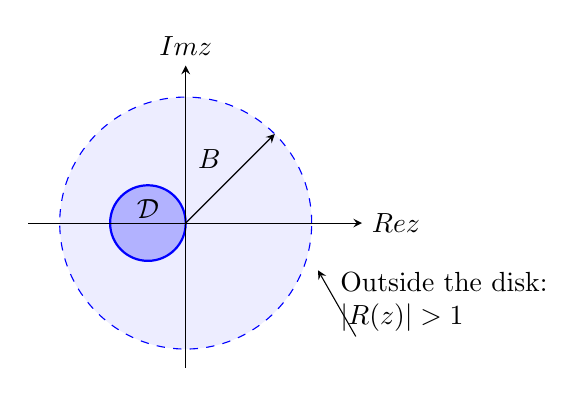
\begin{tikzpicture}[scale=.8,>=stealth]
 \filldraw[fill=blue!7,draw=blue,dashed] (0,0) circle (2);
 \filldraw[fill=blue!30,draw=blue,thick] (-.6,0) circle (.6);
 \draw[->] (-2.5,0)--(2.8,0) node[right] {\(\operatorname{Re}z\)};
 \draw[->] (0,-2.3)--(0,2.5) node[above] {\(\operatorname{Im}z\)};
 \draw[->] (0,0)--(1.414,1.414) node[midway,above left] {\(B\)};
 \node at (-.6,.23) {\(\mathcal D\)};
 \node[align=left] at (4.1,-1.25) {Outside the disk:\\ \(|R(z)|>1\)};
 \draw[->] (2.7,-1.8)--(2.1,-.75);
\end{tikzpicture}
\caption{The polynomial's leading term dominates in every complex
direction. The small region is schematic; the enclosing radius depends
on the method's coefficients and need not be sharp.}
\end{figure}

\begin{remark}[Scope of the theorem]
 The radius may change with \(s\) and with the RK coefficients; the
 theorem does not give one common bound for all explicit methods.
 Consistency rules out the degenerate constant polynomial \(R\equiv1\),
 whose non-strict domain would be all of \(\bb{C}\).
 Implicit methods generally have rational stability functions and can
 have unbounded domains, as the next lecture shows.
\end{remark}

\subsection{A system with a fast decaying mode}

Consider the example from class,
\begin{equation}\label{eq:stiff-matrix-sep-16}
 x'=Ax,\qquad
 A=\begin{bmatrix}0&1\\-50&-51\end{bmatrix}.
\end{equation}
Its characteristic polynomial is
\[
 \det(\lambda I-A)=\lambda^2+51\lambda+50
       =(\lambda+1)(\lambda+50).
\]
With eigenvectors \(v_1=(1,-1)^{\mathsf T}\) and
\(v_2=(1,-50)^{\mathsf T}\), the exact solution is
\[
 x(t)=c_1e^{-t}v_1+c_2e^{-50t}v_2.
\]
Both modes decay, but on very different time scales: \(1\) and
\(1/50\). Forward Euler must satisfy both
\[
 |1-\tau|<1,\qquad |1-50\tau|<1,
\]
so its strict stability restriction is
\begin{equation}\label{eq:stiff-step-bound-sep-16}
 \boxed{0<\tau<\frac1{25}=0.04.}
\end{equation}
At \(\tau=0.04\), the fast numerical mode has multiplier \(-1\)
and fails to decay. Since this matrix is diagonalizable, the endpoint
still gives bounded linear iterates. For \(\tau>0.04\), the fast mode
is unstable. The second-order, two-stage explicit method has exactly
the same restriction because its real stability interval is also
\((-2,0)\).

\begin{figure}[htbp]
\centering
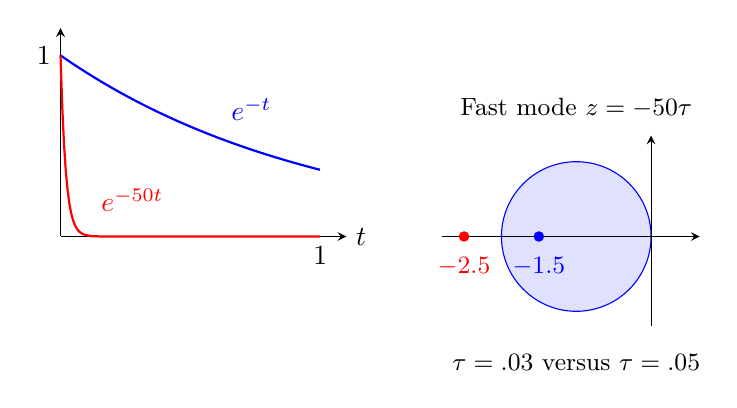
\begin{tikzpicture}[>=stealth]
 \begin{scope}[xscale=3.3,yscale=2.3]
  \draw[->] (0,0)--(1.1,0) node[right] {\(t\)};
  \draw[->] (0,0)--(0,1.15);
  \draw[blue,thick,domain=0:1,samples=100] plot (\x,{exp(-\x)});
  \draw[red,thick,domain=0:1,samples=150] plot (\x,{exp(-50*\x)});
  \node[blue,right] at (.62,.7) {\(e^{-t}\)};
  \node[red,right] at (.12,.2) {\(e^{-50t}\)};
  \node[left] at (0,1) {1}; \node[below] at (1,0) {1};
 \end{scope}
 \begin{scope}[xshift=7.5cm,scale=.95]
  \filldraw[fill=blue!12,draw=blue] (-1,0) circle (1);
  \draw[->] (-2.8,0)--(.65,0);
  \draw[->] (0,-1.2)--(0,1.35);
  \fill[blue] (-1.5,0) circle (2pt);
  \node[blue,below] at (-1.5,-.15) {\small \(-1.5\)};
  \fill[red] (-2.5,0) circle (2pt);
  \node[red,below] at (-2.5,-.15) {\small \(-2.5\)};
  \node[above,align=center] at (-1,1.45) {\small Fast mode \(z=-50\tau\)};
  \node[below] at (-1,-1.45) {\small \(\tau=.03\) versus \(\tau=.05\)};
 \end{scope}
\end{tikzpicture}
\caption{The fast exact mode quickly disappears, but it still limits
Euler's step size. For \(\tau=.03\), its scaled eigenvalue is inside
the disk; for \(\tau=.05\), it is outside.}
\end{figure}

This is the mechanism of \emph{stiffness}: stability requires a much
smaller step than is needed to resolve the slowly varying solution
of interest. Even after the fast exact mode becomes negligible,
roundoff and other perturbations can excite its unstable numerical
counterpart. Stiffness depends on time scales and the integration
interval, not merely on the numerical size of a dimensional eigenvalue.

\subsection{The same restriction near a nonlinear equilibrium}

The nonlinear example in the notes is
\begin{equation}\label{eq:nonlinear-stiff-example-sep-16}
 x'=f(x),\qquad
 f(x_1,x_2)=
 \begin{bmatrix}x_2\\-51x_2-25(x_1^3-x_1)\end{bmatrix}.
\end{equation}
At \(x_*=(1,0)\), \(f(x_*)=0\), and
\[
 Df(x)=\begin{bmatrix}0&1\\-25(3x_1^2-1)&-51\end{bmatrix},
 \qquad Df(1,0)=\begin{bmatrix}0&1\\-50&-51\end{bmatrix}.
\]
The equilibrium is locally asymptotically stable because the Jacobian
has eigenvalues \(-1,-50\).

Euler's map is \(\Psi^\tau(x)=x+\tau f(x)\). It fixes \(x_*\), and
\[
 D\Psi^\tau(x_*)=I+\tau Df(x_*).
\]
For \(0<\tau<1/25\), both multipliers are strictly inside the unit
circle, so the discrete equilibrium is locally asymptotically stable.
The same conclusion holds for explicit RK2, since the derivative of
its map at an equilibrium is \(R_2(\tau Df(x_*))\). At the boundary,
linearization alone does not determine nonlinear stability.

As an additional illustration, write \(q=x_1\), \(v=x_2\). The system
is a damped particle in the potential
\[
 U(q)=\frac{25}{4}(q^2-1)^2,
 \qquad E(q,v)=\frac12v^2+U(q),
 \qquad \frac{dE}{dt}=-51v^2\leq0.
\]
The two potential wells correspond to \((\pm1,0)\); the equilibrium
\((0,0)\) is a saddle because its Jacobian has negative determinant.

\begin{figure}[htbp]
\centering
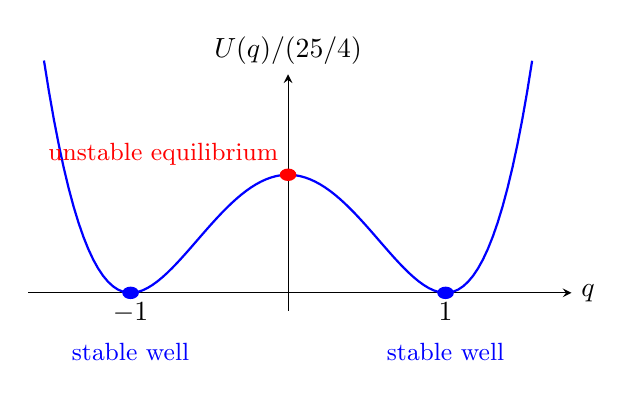
\begin{tikzpicture}[xscale=2,yscale=1.5,>=stealth]
 \draw[->] (-1.65,0)--(1.8,0) node[right] {\(q\)};
 \draw[->] (0,-.15)--(0,1.85) node[above] {\(U(q)/(25/4)\)};
 \draw[blue,thick,domain=-1.55:1.55,samples=100]
  plot (\x,{(\x*\x-1)^2});
 \fill[blue] (-1,0) circle (1.5pt); \fill[blue] (1,0) circle (1.5pt);
 \fill[red] (0,1) circle (1.5pt);
 \node[below] at (-1,0) {\(-1\)}; \node[below] at (1,0) {1};
 \node[above left,red] at (0,1) {\small unstable equilibrium};
 \node[blue] at (1,-.5) {\small stable well};
 \node[blue] at (-1,-.5) {\small stable well};
\end{tikzpicture}
\caption{The potential of the nonlinear example. Damping decreases
mechanical energy; the Jacobian gives the local decay rates near a well.}
\end{figure}

\subsection{An oscillator: forward Euler is never stable}

For
\begin{equation}\label{eq:oscillator-sep-16}
 x'=Ax,\qquad A=\begin{bmatrix}0&1\\-1&0\end{bmatrix},
\end{equation}
the eigenvalues are \(\pm i\). Since \(A^{\mathsf T}=-A\),
\[
 \frac{d}{dt}\|x(t)\|_2^2=0.
\]
The exact trajectories are circles, and the origin is stable but not
asymptotically stable. Forward Euler has eigenvalues \(1\pm i\tau\),
whose modulus is \(\sqrt{1+\tau^2}>1\) for every \(\tau>0\).
Equivalently,
\[
 (I+\tau A)^{\mathsf T}(I+\tau A)=(1+\tau^2)I,
 \qquad
 \|x_n\|_2=(1+\tau^2)^{n/2}\|x_0\|_2.
\]
Thus every positive fixed step causes artificial growth over long
integration times. This does not contradict convergence as
\(\tau\to0\) on a fixed finite time interval.

\begin{figure}[htbp]
\centering
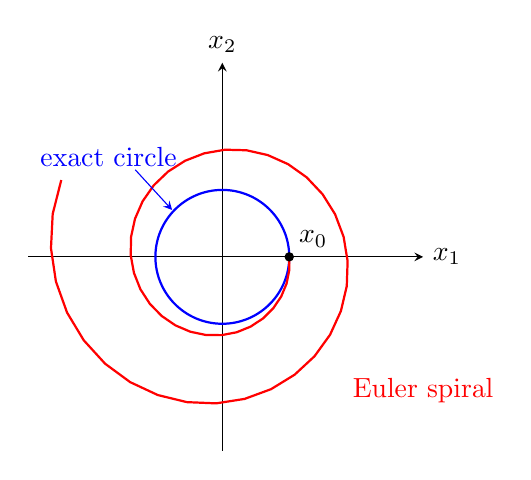
\begin{tikzpicture}[scale=.85,>=stealth]
 \draw[->] (-2.9,0)--(3,0) node[right] {\(x_1\)};
 \draw[->] (0,-2.9)--(0,2.9) node[above] {\(x_2\)};
 \draw[blue,thick] (0,0) circle (1);
 \draw[red,thick] plot coordinates {
(1.00000,0.00000) (1.00000,-0.20000) (0.96000,-0.40000) (0.88000,-0.59200) (0.76160,-0.76800) (0.60800,-0.92032)
(0.42394,-1.04192) (0.21555,-1.12671) (-0.00979,-1.16982) (-0.24375,-1.16786) (-0.47732,-1.11911) (-0.70115,-1.02364)
(-0.90588,-0.88341) (-1.08256,-0.70224) (-1.22301,-0.48573) (-1.32015,-0.24113) (-1.36838,0.02290) (-1.36380,0.29658)
(-1.30448,0.56934) (-1.19061,0.83023) (-1.02457,1.06836) (-0.81089,1.27327) (-0.55624,1.43545) (-0.26915,1.54670)
(0.04019,1.60053) (0.36029,1.59249) (0.67879,1.52043) (0.98288,1.38467) (1.25981,1.18810) (1.49743,0.93613)
(1.68466,0.63665) (1.81199,0.29972) (1.87193,-0.06268) (1.85940,-0.43707) (1.77198,-0.80895) (1.61019,-1.16334)
(1.37752,-1.48538) (1.08045,-1.76089) (0.72827,-1.97698) (0.33287,-2.12263) (-0.09165,-2.18921) (-0.52949,-2.17088)
(-0.96367,-2.06498) (-1.37666,-1.87224) (-1.75111,-1.59691) (-2.07049,-1.24669) (-2.31983,-0.83259) (-2.48635,-0.36862)
(-2.56007,0.12865) (-2.53434,0.64066) (-2.40621,1.14753)};
 \fill (1,0) circle (2pt) node[above right] {\(x_0\)};
 \node[blue] at (-1.7,1.5) {exact circle};
 \draw[blue,->] (-1.3,1.3)--(-.75,.7);
 \node[red] at (3,-2) {Euler spiral};
\end{tikzpicture}
\caption{Forward Euler on the oscillator, starting at \((1,0)\), with
\(\tau=.2\) for 50 steps. The exact orbit has radius one; the numerical
radius grows by \(\sqrt{1+\tau^2}\) at each step.}
\end{figure}

For comparison, direct calculation gives
\begin{align*}
 |R_2(iy)|^2&=1+\frac{y^4}{4},\\*
 |R_3(iy)|^2&=1+\frac{y^4(y^2-3)}{36},\\*
 |R_4(iy)|^2&=1+\frac{y^6(y^2-8)}{576}.
\end{align*}
Hence RK2 is also unstable on this oscillator for every \(\tau>0\).
RK3 and RK4 have bounded iterates for
\(0<\tau\leq\sqrt3\) and \(0<\tau\leq2\sqrt2\), respectively.
Inside these intervals their amplification factors have modulus less
than one, so they introduce numerical damping. Stability alone does
not imply preservation of the exact oscillation amplitude or phase.
